\documentclass[letterpaper, 10 pt, conference]{ieeeconf}

\IEEEoverridecommandlockouts
\overrideIEEEmargins

\usepackage[utf8]{inputenc}
\usepackage[T1]{fontenc}
\usepackage{amsmath}
\usepackage{amssymb}
\usepackage{booktabs}
\usepackage{cite}
\usepackage{graphicx}
\usepackage{multirow}
\usepackage{xcolor}
\usepackage{url}

\newcommand{\method}{ForeTac}
\newcommand{\Real}{\mathbb{R}}
\newcommand{\loss}{\mathcal{L}}
\newcommand{\marker}{\mathbf{m}}
\newcommand{\action}{\mathbf{a}}
\newcommand{\obs}{\mathbf{o}}
\newcommand{\latent}{\mathbf{z}}
\newcommand{\score}{S}

\title{\LARGE \bf
ForeTac: Steering Robot Actions with Predicted Contact Consequences}

% RA-L initial submissions are double-anonymous.
\author{Anonymous Authors}

\begin{document}

\maketitle
\thispagestyle{empty}
\pagestyle{empty}

\begin{abstract}
Contact-rich manipulation requires decisions about physical interaction before
the relevant tactile evidence is fully observed. A visually plausible motion can
still lose contact during wiping, overload a fragile object, collide with a
slot edge, or jam during insertion. This paper presents \method{}, a framework
for steering robot action chunks with predicted contact consequences. A base
Diffusion Policy proposes an action chunk from visual, proprioceptive, and
tactile observations. An action-conditioned tactile foresight model predicts the
future GelSight marker-field latent sequence induced by the candidate chunk. A
contact-quality energy model then scores the predicted tactile future, and its
gradient is used for bounded trust-region refinement during late denoising. The
result is a modular inference-time contact signal: the base policy remains the
behavioral prior, while predicted tactile consequences provide a proactive
correction before execution. We instantiate \method{} on five real-robot
contact tasks: board wiping, vase wiping, card swiping, chip grasping, and
socket insertion. Current experiments validate the tactile latent
representation, multi-horizon foresight accuracy, and bounded guidance
gradients on blackboard wiping; paired online success-rate comparisons are
specified as the remaining controlled rollout study.
\end{abstract}

\vspace{0.5em}
\noindent\textbf{Index Terms}--Contact-rich manipulation, tactile sensing,
diffusion policy, tactile foresight, inference-time guidance.

\section{INTRODUCTION}

The central difficulty in contact-rich robot manipulation is that the outcome of
an action is not fully determined by its geometric path. The same end-effector
trajectory can be successful, ineffective, or unsafe depending on contact
pressure, shear, impact, slip, and the temporal stability of those quantities.
This distinction is easy to miss in tasks that look visually simple. In board
wiping, a motion can cover the intended region while applying too little force
to clean the surface or too much force for safe execution. In vase wiping, the
same issue is compounded by a curved and fragile object. In card swiping,
success requires sustained sliding contact through a narrow slot rather than
merely reaching the slot entrance. In chip grasping, a small increase in
pressure can break the object. In socket insertion, a small lateral contact
before alignment can create bounce, jamming, or repeated retries. These
examples share a common structure: the robot must choose an action based on the
contact consequence it will create, not only on the current visual state.

Recent imitation-learning policies have substantially improved the action
generation side of robotic manipulation. Action Chunking Transformers and
Diffusion Policy learn expressive multi-step action distributions from
demonstrations and can produce smooth behavior over long horizons
\cite{zhao2023act,chi2023diffusion}. Their strength, however, also reveals a
limitation. A policy trained to imitate successful trajectories may still make
small local contact mistakes at deployment, especially when the object pose,
surface normal, friction, or initial contact condition differs from the
demonstrations. Adding tactile observations to the policy can improve the
current state estimate \cite{calandra2018more,lee2019making,li2022see}, but
standard tactile fusion remains mostly reactive: the robot observes contact
after it happens and then changes future actions. For delicate contact, the
critical decision often comes earlier. Before executing an action chunk, the
robot should ask: if this candidate action is taken, what tactile state will it
produce, and is that future contact desirable?

This question motivates a research gap between three lines of work that have
largely remained separate. First, tactile representation learning provides
compact encodings of high-dimensional touch signals
\cite{higuera2024sparsh,zhao2024t3}. These representations improve perception,
but by themselves do not decide how a candidate action should change. Second,
visuo-tactile or visual world models predict future sensory states
\cite{ebert2018visual,ye2025dreamtacvla,zheng2026omnivta,higuera2026vtwm}.
Prediction is useful, but many systems use it as an auxiliary training signal,
a latent feature, or a planning model without an explicit differentiable link
from predicted tactile quality back to the sampled action. Third,
inference-time guidance and energy-based action selection can steer diffusion
policies or rerank candidates \cite{florence2021ibc,du2025dynaguide,
saxena2025sitcom,zhang2026touchguide}. Yet contact-rich manipulation needs a
specific kind of guidance: the score should be grounded in the tactile future
that the action itself is predicted to cause, and the update must stay close to
the demonstrated behavior manifold so that the scorer cannot exploit
out-of-distribution actions.

\method{} is designed to close this gap. The framework treats future tactile
consequences as an action-quality signal. At each control step, a base
Diffusion Policy proposes an action chunk. A tactile foresight transformer then
predicts a future sequence of GelSight marker-field latents conditioned on the
candidate action. A contact-quality energy model scores the predicted future
for task-appropriate contact. During selected late denoising steps, \method{}
backpropagates this score through the foresight model to the action sample and
applies a small trust-region update. This converts tactile foresight from a
passive prediction target into an active inference-time correction.

The design intentionally separates the roles of the modules. The diffusion
policy is responsible for producing actions on the demonstration manifold. The
foresight model is responsible for answering the counterfactual contact
question: what tactile sequence is likely under this action? The energy scorer
is responsible for distinguishing useful contact from task-specific failure
modes such as contact loss, overload, pressure instability, slip, bounce, and
jamming. The trust-region update is responsible for making only bounded local
changes. This modularity is important academically and practically: it turns
contact quality into an explicit testable object, allows independent evaluation
of representation, prediction, scoring, and guidance, and avoids conflating
better policy training with better inference-time contact reasoning.

This paper makes the following contributions.
\begin{itemize}
\item We formulate contact-rich action selection as prediction-conditioned
guidance: actions are evaluated by the tactile consequences they are predicted
to create, rather than only by their current observation likelihood.
\item We introduce an action-conditioned multi-step tactile foresight module
over compact TacVAE marker-field latents, preserving the temporal information
needed to detect contact dropout, pressure spikes, and unstable force.
\item We use a contact-quality energy model trained with semantic failure
labels and deploy its margin score as a differentiable guidance signal for
late-stage diffusion denoising.
\item We define a five-task real-robot evaluation suite and report current
evidence for tactile reconstruction, foresight prediction, and bounded guidance
diagnostics, while explicitly separating these offline results from the pending
paired online success-rate study.
\end{itemize}

\begin{figure*}[t]
  \centering
  
\includegraphics[width=0.92\textwidth]{figures/teaser.png}
  \caption{\textbf{\method{} overview.} The robot predicts future tactile
  consequences of candidate action chunks, scores the predicted contact quality,
  and applies a bounded correction before execution. The same predict-score-guide
  structure applies across wiping, swiping, grasping, and insertion tasks.}
  \label{fig:teaser}
\end{figure*}

\section{RELATED WORK}

\subsection{Action-Chunk Policies for Robot Manipulation}

Action-chunk policies reduce compounding errors by predicting a sequence of
future controls rather than a single next action. ACT uses a transformer policy
to predict smooth action chunks from demonstrations \cite{zhao2023act}.
Diffusion Policy models the action chunk distribution with conditional
denoising and has become a strong visuomotor imitation baseline
\cite{chi2023diffusion}. Follow-up work improves 3D representations and
sampling efficiency \cite{ze2024dp3,prasad2024consistency}. \method{} is
compatible with these policies because it does not replace the base action
generator. It adds a local contact-quality objective during inference.

\subsection{Tactile Representation and Prediction}

Vision-based tactile sensors reveal local deformation, shear, and pressure that
are difficult to infer from RGB images alone \cite{calandra2018more,
lee2019making,li2022see}. Learned tactile representations such as Sparsh and
T3 provide transferable features for touch \cite{higuera2024sparsh,
zhao2024t3}. Visuo-tactile world models and tactile prediction methods further
learn how touch evolves under actions \cite{ye2025dreamtacvla,
zheng2026omnivta,higuera2026vtwm,niu2026htd}. Our focus is not only to predict
touch, but to use predicted touch as an explicit differentiable action-quality
signal.

\subsection{Inference-Time Guidance and Candidate Verification}

Energy-based imitation and candidate verification methods improve robot action
selection by scoring or steering samples \cite{florence2021ibc,
saxena2025sitcom}. DynaGuide uses dynamics-based guidance for diffusion
policies \cite{du2025dynaguide}, and touch-based guidance explores
inference-time tactile steering \cite{zhang2026touchguide}. \method{} differs
in the source of the score. The score is computed from the future tactile
consequence predicted for the current candidate action and is injected through a
bounded update, rather than selecting a full trajectory only after sampling.

\section{PROBLEM FORMULATION}

At time $t$, the robot observes
\begin{equation}
\obs_t = \{I_t^g, I_t^w, q_t, \marker_{t-W+1:t}\},
\end{equation}
where $I_t^g$ and $I_t^w$ are global and wrist images, $q_t \in \Real^{d_q}$ is
the robot state, and $\marker_{t-W+1:t}$ is a recent tactile marker history. The
base policy generates an action chunk
\begin{equation}
\action_{t:t+H-1} \in \Real^{H \times d_a}.
\end{equation}
The goal is to choose a chunk that both remains likely under the demonstration
policy and produces high-quality future contact.

Let $E_{\rm tac}$ encode tactile marker histories into latent maps and let
$f_\psi$ be the action-conditioned tactile foresight model:
\begin{equation}
\hat{\latent}_{t:t+H_f-1}
= f_\psi(\obs_t,\action_{t:t+H_f-1}).
\end{equation}
A contact-quality scorer returns
\begin{equation}
s = \score_\phi(\action_{t:t+H_f-1},
\hat{\latent}_{t:t+H_f-1},\tau),
\end{equation}
where $\tau$ denotes the task or contact-quality semantics. \method{} locally
improves the diffusion action prior with the predicted-contact objective:
\begin{equation}
\log p_\theta(\action_{t:t+H-1}|\obs_t)
+ \lambda \score_\phi(\action,f_\psi(\obs_t,\action),\tau).
\end{equation}
The second term is not optimized freely. It is used as a small late-denoising
correction so that the base policy remains the main behavioral prior.

\section{METHOD}

\subsection{System Overview}

\method{} has four stages. First, a TacVAE compresses tactile marker histories
into structured latent maps. Second, a base Diffusion Policy learns the action
prior from demonstrations. Third, a foresight transformer predicts future
tactile latents from the current observation and candidate action chunk. Fourth,
a contact-quality energy model scores the predicted tactile future and supplies
an inference-time guidance gradient.

\begin{figure}[t]
  \centering
  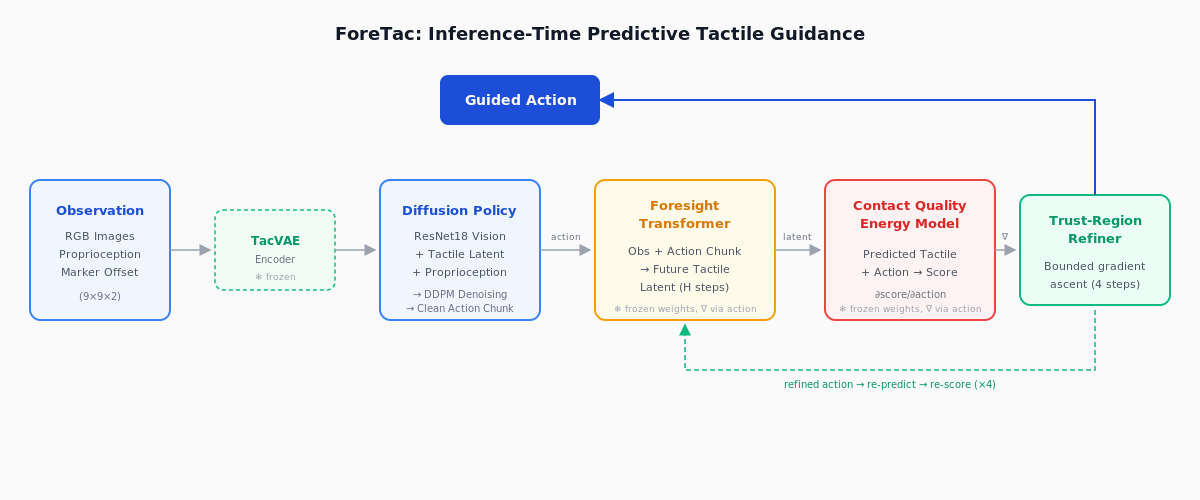
\includegraphics[width=0.98\linewidth]{figures/architecture.png}
  \caption{\textbf{Architecture.} A base Diffusion Policy proposes an action
  chunk. Tactile foresight predicts the contact consequence of the chunk. A
  contact-quality energy model scores the prediction and sends a bounded
  gradient back to the action sample.}
  \label{fig:architecture}
\end{figure}

\subsection{TacVAE Marker-Field Latents}

The GelSight marker field is represented as a $9 \times 9 \times 2$ displacement
grid. TacVAE encodes a recent marker history into a compact spatial latent
\begin{equation}
\latent_t = E_{\rm tac}(\marker_{t-W+1:t})
\in \Real^{16 \times 3 \times 3}.
\end{equation}
The latent is flattened to 144 dimensions for foresight and scoring. The
decoder maps latents back to marker displacement fields for reconstruction and
prediction diagnostics. This representation preserves spatial contact structure
while avoiding direct prediction in a noisy raw marker space.

\subsection{Action-Conditioned Tactile Foresight}

The foresight model predicts the tactile sequence induced by a candidate action
chunk:
\begin{equation}
\hat{\latent}_{t:t+H_f-1}
= f_\psi(\latent_t,q_t,\action_{t:t+H_f-1}).
\end{equation}
The current implementation uses $H_f=16$ for the main board setting. Predicting
a sequence rather than a single endpoint is important because contact quality is
temporal: a transient pressure spike, contact loss, or oscillation can make an
otherwise plausible trajectory unsafe.

Training uses future TacVAE latents as targets. The loss combines latent
prediction, decoded-marker reconstruction, and temporal-difference consistency:
\begin{equation}
\loss_{\rm fs}
= \loss_{\rm latent}
+ \lambda_m \loss_{\rm marker}
+ \lambda_\Delta \loss_\Delta .
\end{equation}
For stride-aligned deployment, action and tactile target indices are sampled
with the same temporal stride so that training and serving contracts match.

\subsection{Contact-Quality Energy}

The contact-quality scorer converts the predicted tactile future into a scalar
score. Rather than hand-coding one force threshold, the scorer is trained with
semantic contact labels. For board wiping, the labels are expert contact,
pressure too small, pressure too large, and pressure unstable. For insertion,
negative modes include pre-bounce, bounce, edge contact, and jamming. For vase
wiping, card swiping, and chip grasping, the same structure is reused with
task-specific labels such as contact dropout, slip, overload, and excessive
object disturbance.

The deployed score is an unsaturated logit margin:
\begin{equation}
s_{\rm margin}
= \ell_{\rm good}
- \log \sum_{c \in \mathcal{C}_{\rm bad}} \exp(\ell_c),
\label{eq:margin}
\end{equation}
where $\ell_c$ is the class logit for contact class $c$. The margin is preferred
over a saturated good-contact probability because it provides usable gradients
even when the classifier is confident.

\subsection{Trust-Region Denoising Guidance}

Diffusion Policy denoises an action sample $x_i$ at diffusion step $i$. From
the predicted noise $\epsilon_\theta(x_i,i,\obs_t)$, the clean-action estimate
is
\begin{equation}
\hat{x}_0 =
\frac{x_i-\sqrt{1-\bar{\alpha}_i}\epsilon_\theta(x_i,i,\obs_t)}
{\sqrt{\bar{\alpha}_i}}.
\label{eq:x0}
\end{equation}
At selected late denoising steps, \method{} denormalizes $\hat{x}_0$, predicts
future tactile latents, computes the contact-quality score, and backpropagates:
\begin{equation}
g_i = \nabla_{x_i}
\score_\phi(\hat{x}_0,f_\psi(\obs_t,\hat{x}_0),\tau).
\end{equation}
The sample is updated by a bounded normalized step:
\begin{equation}
x_i \leftarrow x_i +
\eta \frac{g_i}{\|g_i\|_2+\epsilon},
\label{eq:guidance}
\end{equation}
followed by trust-region checks in raw action units. In the main latent-only
guidance path, the action branch of the scorer is detached so that the cleanest
gradient route is
\begin{equation}
\action \rightarrow \hat{\latent}_{t:t+H_f-1}
\rightarrow \score_\phi.
\end{equation}
This reduces the chance that the scorer exploits an action-only shortcut and
keeps the guidance grounded in predicted tactile consequences.

\begin{figure}[t]
  \centering
  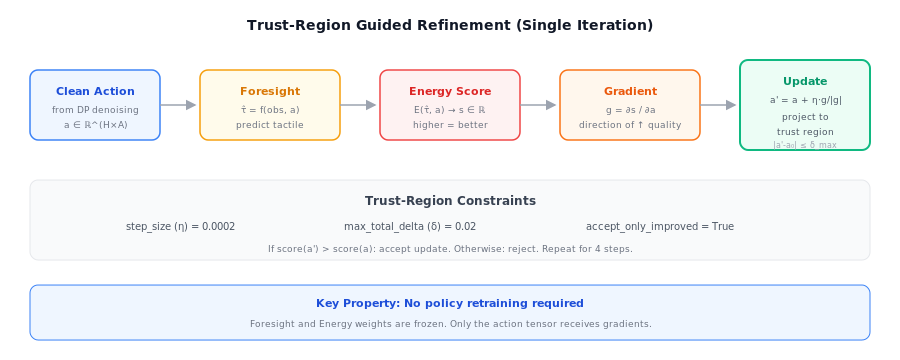
\includegraphics[width=0.98\linewidth]{figures/guidance_mechanism.png}
  \caption{\textbf{Guidance mechanism.} Guidance is applied only during late
  denoising, uses a normalized small step, and accepts bounded corrections that
  improve predicted contact quality.}
  \label{fig:guidance}
\end{figure}

\section{EXPERIMENTAL SETUP}

\subsection{Tasks}

We evaluate \method{} on five contact-rich tasks.
\textbf{Board wiping} requires stable moderate pressure while sweeping across a
flat board.
\textbf{Vase wiping} requires wiping a curved fragile surface without excessive
normal force or object displacement.
\textbf{Card swiping} requires continuous sliding contact and correct slot
alignment.
\textbf{Chip grasping} requires enough force to lift a fragile chip without
crushing it.
\textbf{Socket insertion} requires tight alignment while avoiding side contact,
bounce, and jamming.

\subsection{Baselines and Metrics}

The planned online comparison follows the project page and compares \method{}
against a visual Diffusion Policy (DP), DP with tactile conditioning, a general
VLA policy baseline, a reactive diffusion-transformer baseline, and a foresight
autoregressive baseline. The primary metric is task success. The secondary
metric is safe success, counted only when the task succeeds without unsafe
contact, emergency stops, damaging interactions, or task-specific failure
modes. Additional task metrics include force-band ratio, force variance,
contact-dropout ratio, retry count, bounce count, and peak force.

\begin{table*}[t]
\caption{Planned paired online success-rate comparison. Values are intentionally
left as TBD until controlled baseline-versus-guided real-rollout trials are
completed.}
\label{tab:online}
\centering
\setlength{\tabcolsep}{4pt}
\begin{tabular}{lcccccccccc}
\toprule
\multirow{2}{*}{Method}
& \multicolumn{2}{c}{Board}
& \multicolumn{2}{c}{Vase}
& \multicolumn{2}{c}{Card}
& \multicolumn{2}{c}{Chip}
& \multicolumn{2}{c}{Socket}\\
\cmidrule(lr){2-3}\cmidrule(lr){4-5}\cmidrule(lr){6-7}
\cmidrule(lr){8-9}\cmidrule(lr){10-11}
& Succ. & Safe & Succ. & Safe & Succ. & Safe & Succ. & Safe & Succ. & Safe\\
\midrule
DP & TBD & TBD & TBD & TBD & TBD & TBD & TBD & TBD & TBD & TBD\\
DP + tactile & TBD & TBD & TBD & TBD & TBD & TBD & TBD & TBD & TBD & TBD\\
VLA baseline & TBD & TBD & TBD & TBD & TBD & TBD & TBD & TBD & TBD & TBD\\
Reactive baseline & TBD & TBD & TBD & TBD & TBD & TBD & TBD & TBD & TBD & TBD\\
Foresight autoregressive & TBD & TBD & TBD & TBD & TBD & TBD & TBD & TBD & TBD & TBD\\
\method{} & TBD & TBD & TBD & TBD & TBD & TBD & TBD & TBD & TBD & TBD\\
\bottomrule
\end{tabular}
\end{table*}

\subsection{Offline Evidence Required Before Rollouts}

Before claiming online improvement, we require three checks. First, TacVAE must
reconstruct marker fields accurately enough that downstream prediction preserves
contact magnitude and direction. Second, tactile foresight must predict future
latents and decoded marker fields across the horizons used by the controller.
Third, the scorer must provide finite, bounded, and localized gradients when
composed with the foresight model and the diffusion sampler. These checks do not
replace real-robot success-rate comparisons, but they are necessary for safe and
interpretable deployment.

\section{CURRENT RESULTS}

\subsection{TacVAE Reconstruction}

Table~\ref{tab:tacvae} reports the current TacVAE reconstruction evidence from
the project page. Normalized MAE measures marker-field reconstruction error and
cosine similarity measures directional agreement of the reconstructed tactile
deformation.

\begin{table}[t]
\caption{TacVAE marker-field reconstruction quality. Chip evaluation is pending.}
\label{tab:tacvae}
\centering
\begin{tabular}{lcc}
\toprule
Task & Norm. MAE $\downarrow$ & Cosine $\uparrow$\\
\midrule
Board wiping & 0.039 & 0.998\\
Vase wiping & 0.110 & 0.986\\
Card swiping & 0.039 & 0.998\\
Chip grasping & TBD & TBD\\
Socket insertion & 0.038 & 0.998\\
\bottomrule
\end{tabular}
\end{table}

\subsection{Foresight Prediction Quality}

The board foresight visualization evaluates horizons $H=\{1,4,8,12,16\}$ over
32 validation windows. Latent MAE increases from 0.167 at $H=1$ to 0.274 at
$H=16$, while latent cosine remains high from 0.9993 to 0.9953. Decoded marker
error increases from 0.213 px to 0.377 px across the same horizon range. These
numbers indicate the expected horizon degradation while preserving the
directional structure needed for contact-quality scoring.

\begin{figure}[t]
  \centering
  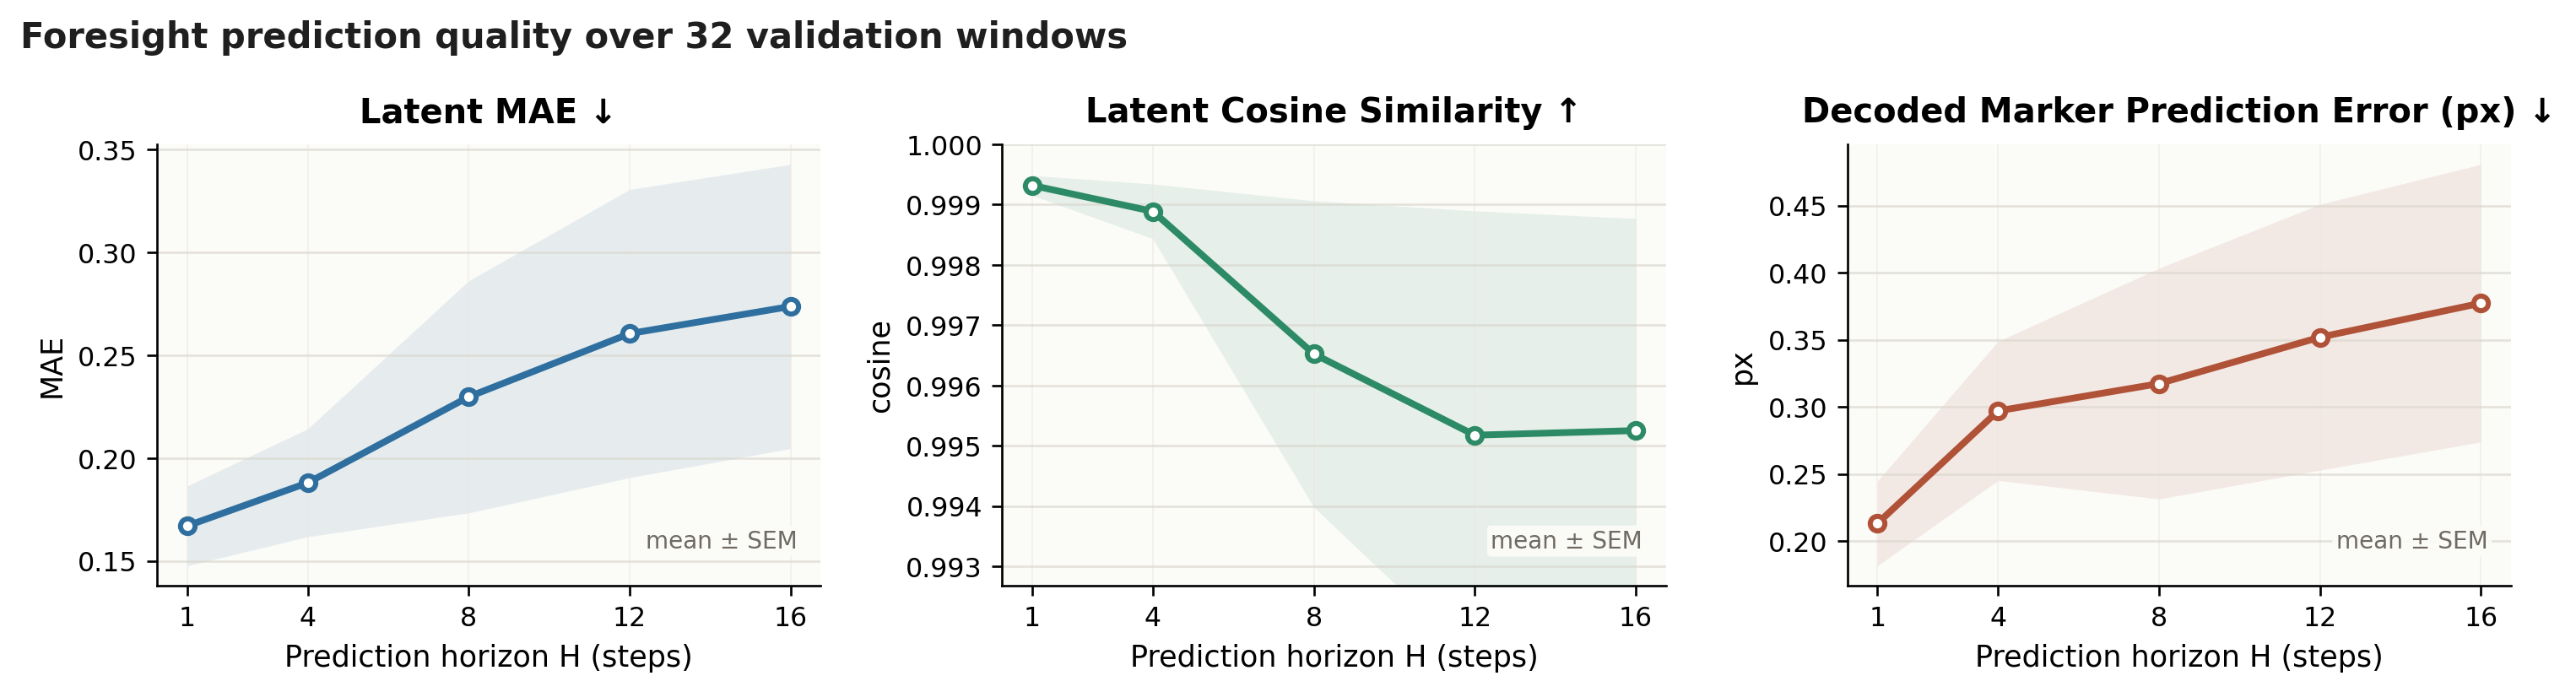
\includegraphics[width=0.98\linewidth]{figures/foresight_prediction_quality_horizons.png}
  \caption{\textbf{Foresight prediction quality.} Tactile foresight is evaluated
  by latent MAE, latent cosine similarity, and decoded marker-field error across
  horizons.}
  \label{fig:foresight_quality}
\end{figure}

\begin{figure}[t]
  \centering
  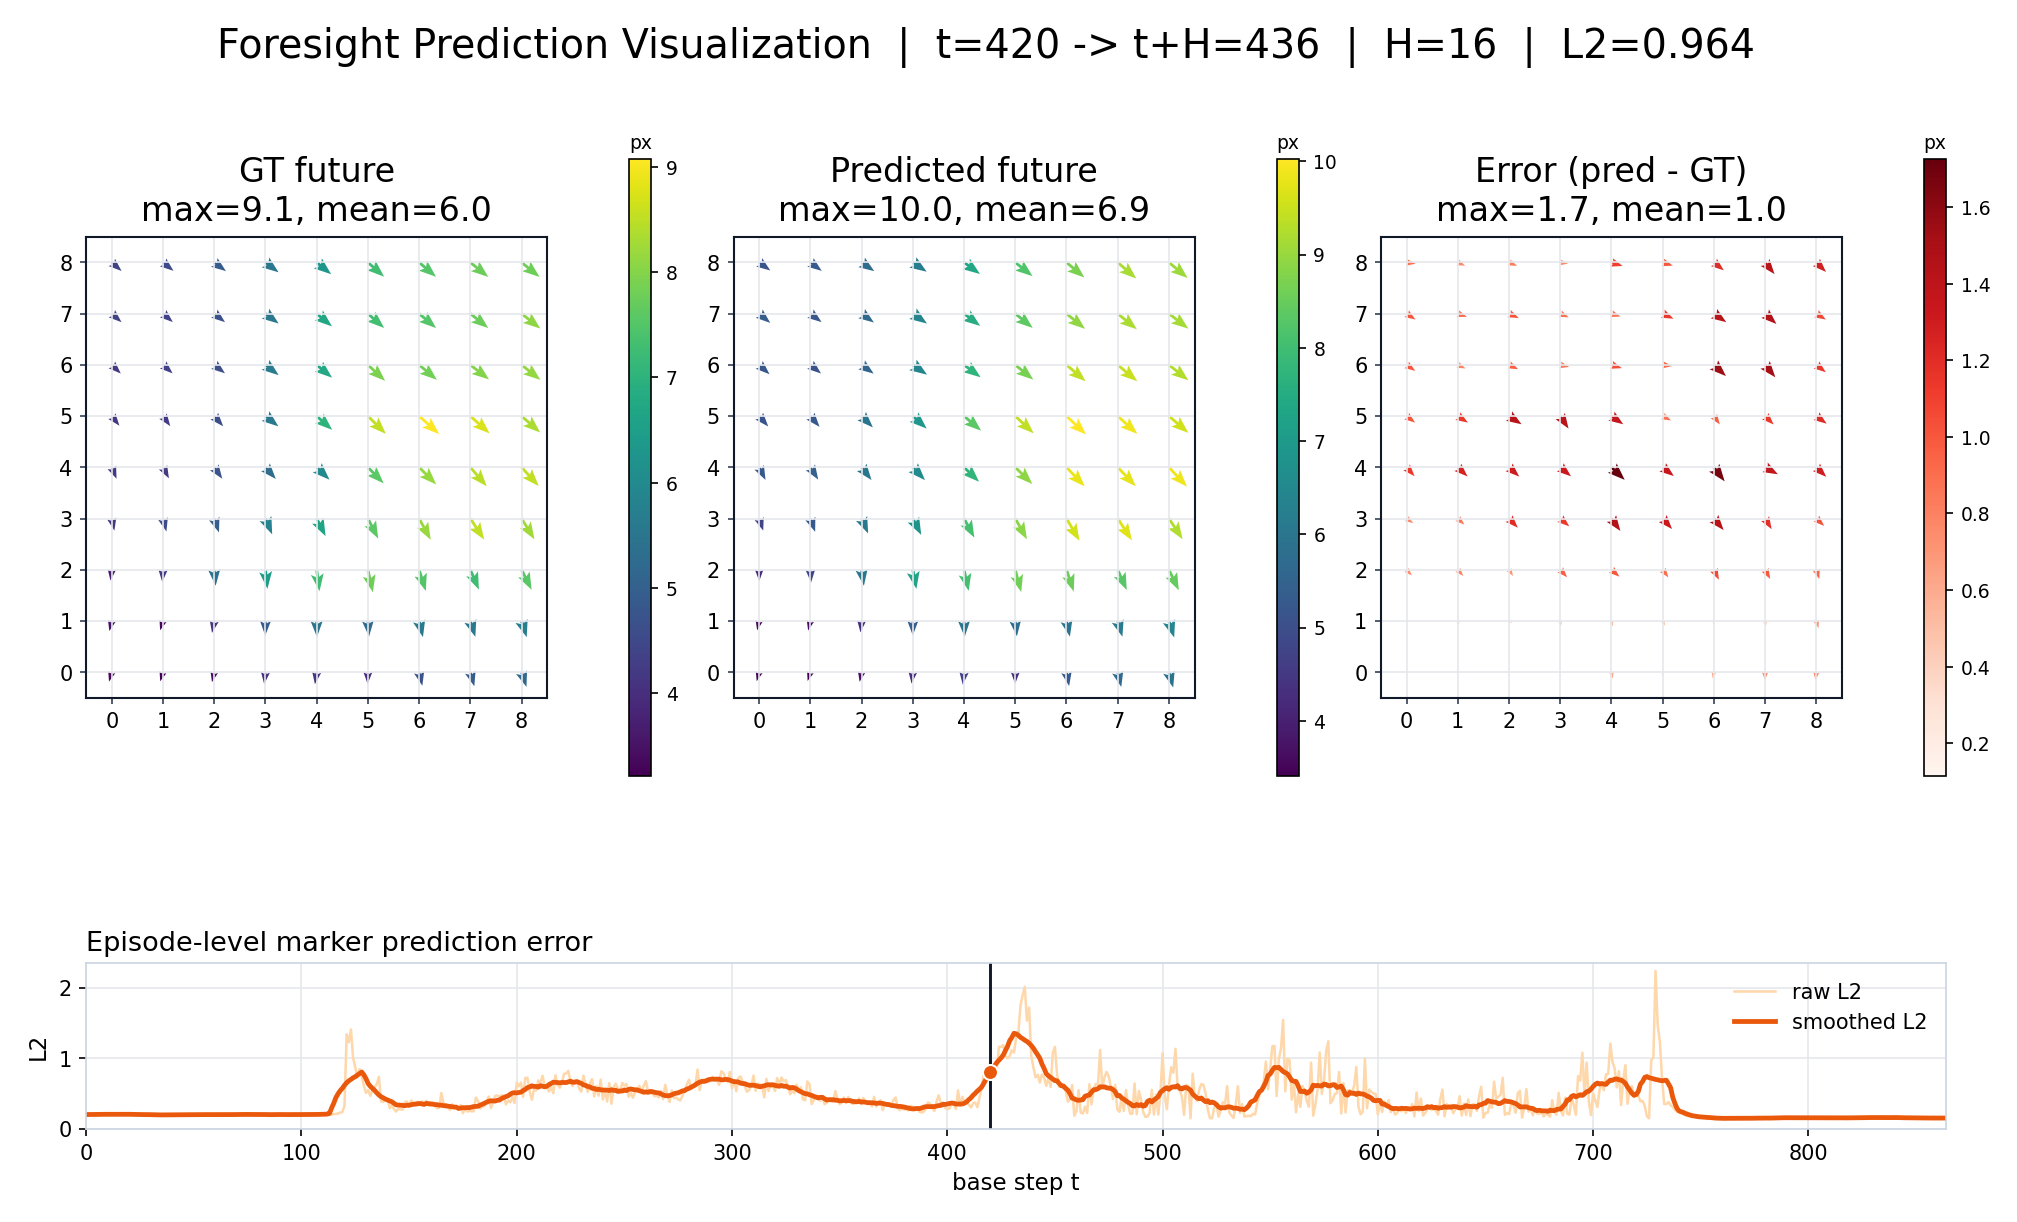
\includegraphics[width=0.98\linewidth]{figures/foresight_prediction_board_episode6_tplus16_summary.png}
  \caption{\textbf{Predicted versus observed tactile consequence.} Example
  board-wiping visualization comparing predicted marker displacement fields with
  ground-truth future observations at the long horizon.}
  \label{fig:foresight_example}
\end{figure}

\subsection{Guidance Diagnostics}

The current blackboard stride-3 diagnostic uses a temporal-stride-aligned
foresight checkpoint and a latent energy scorer with expert-margin score. On the
held-out validation split, the scorer separates expert, pressure-too-small,
pressure-too-large, and pressure-unstable windows with accuracy 1.0,
macro-F1 1.0, expert-vs-negative AUROC 1.0, and expert-margin AUROC 1.0 over
3144 windows. For 128 selected validation windows, all rows produce finite
action gradients. The mean raw gradient norm is 2.4475 and the mean scaled norm
with guidance scale 0.003 is 0.00734. Existing dense denoising logs show a mean
guided-step score delta of 0.0198 with an applied update norm fixed near 0.003.

\begin{table}[t]
\caption{Blackboard stride-3 guidance diagnostic. This is an offline
gradient/sampler check, not an online success-rate result.}
\label{tab:guidance_diag}
\centering
\begin{tabular}{lc}
\toprule
Metric & Value\\
\midrule
Validation windows & 3144\\
Scorer accuracy / macro-F1 & 1.000 / 1.000\\
Expert-margin AUROC & 1.000\\
Rows with finite gradients & 128 / 128\\
Mean raw gradient norm & 2.4475\\
Mean scaled gradient norm & 0.00734\\
Mean guided-step score delta & 0.0198\\
Mean applied update norm & 0.0030\\
\bottomrule
\end{tabular}
\end{table}

\begin{figure*}[t]
  \centering
  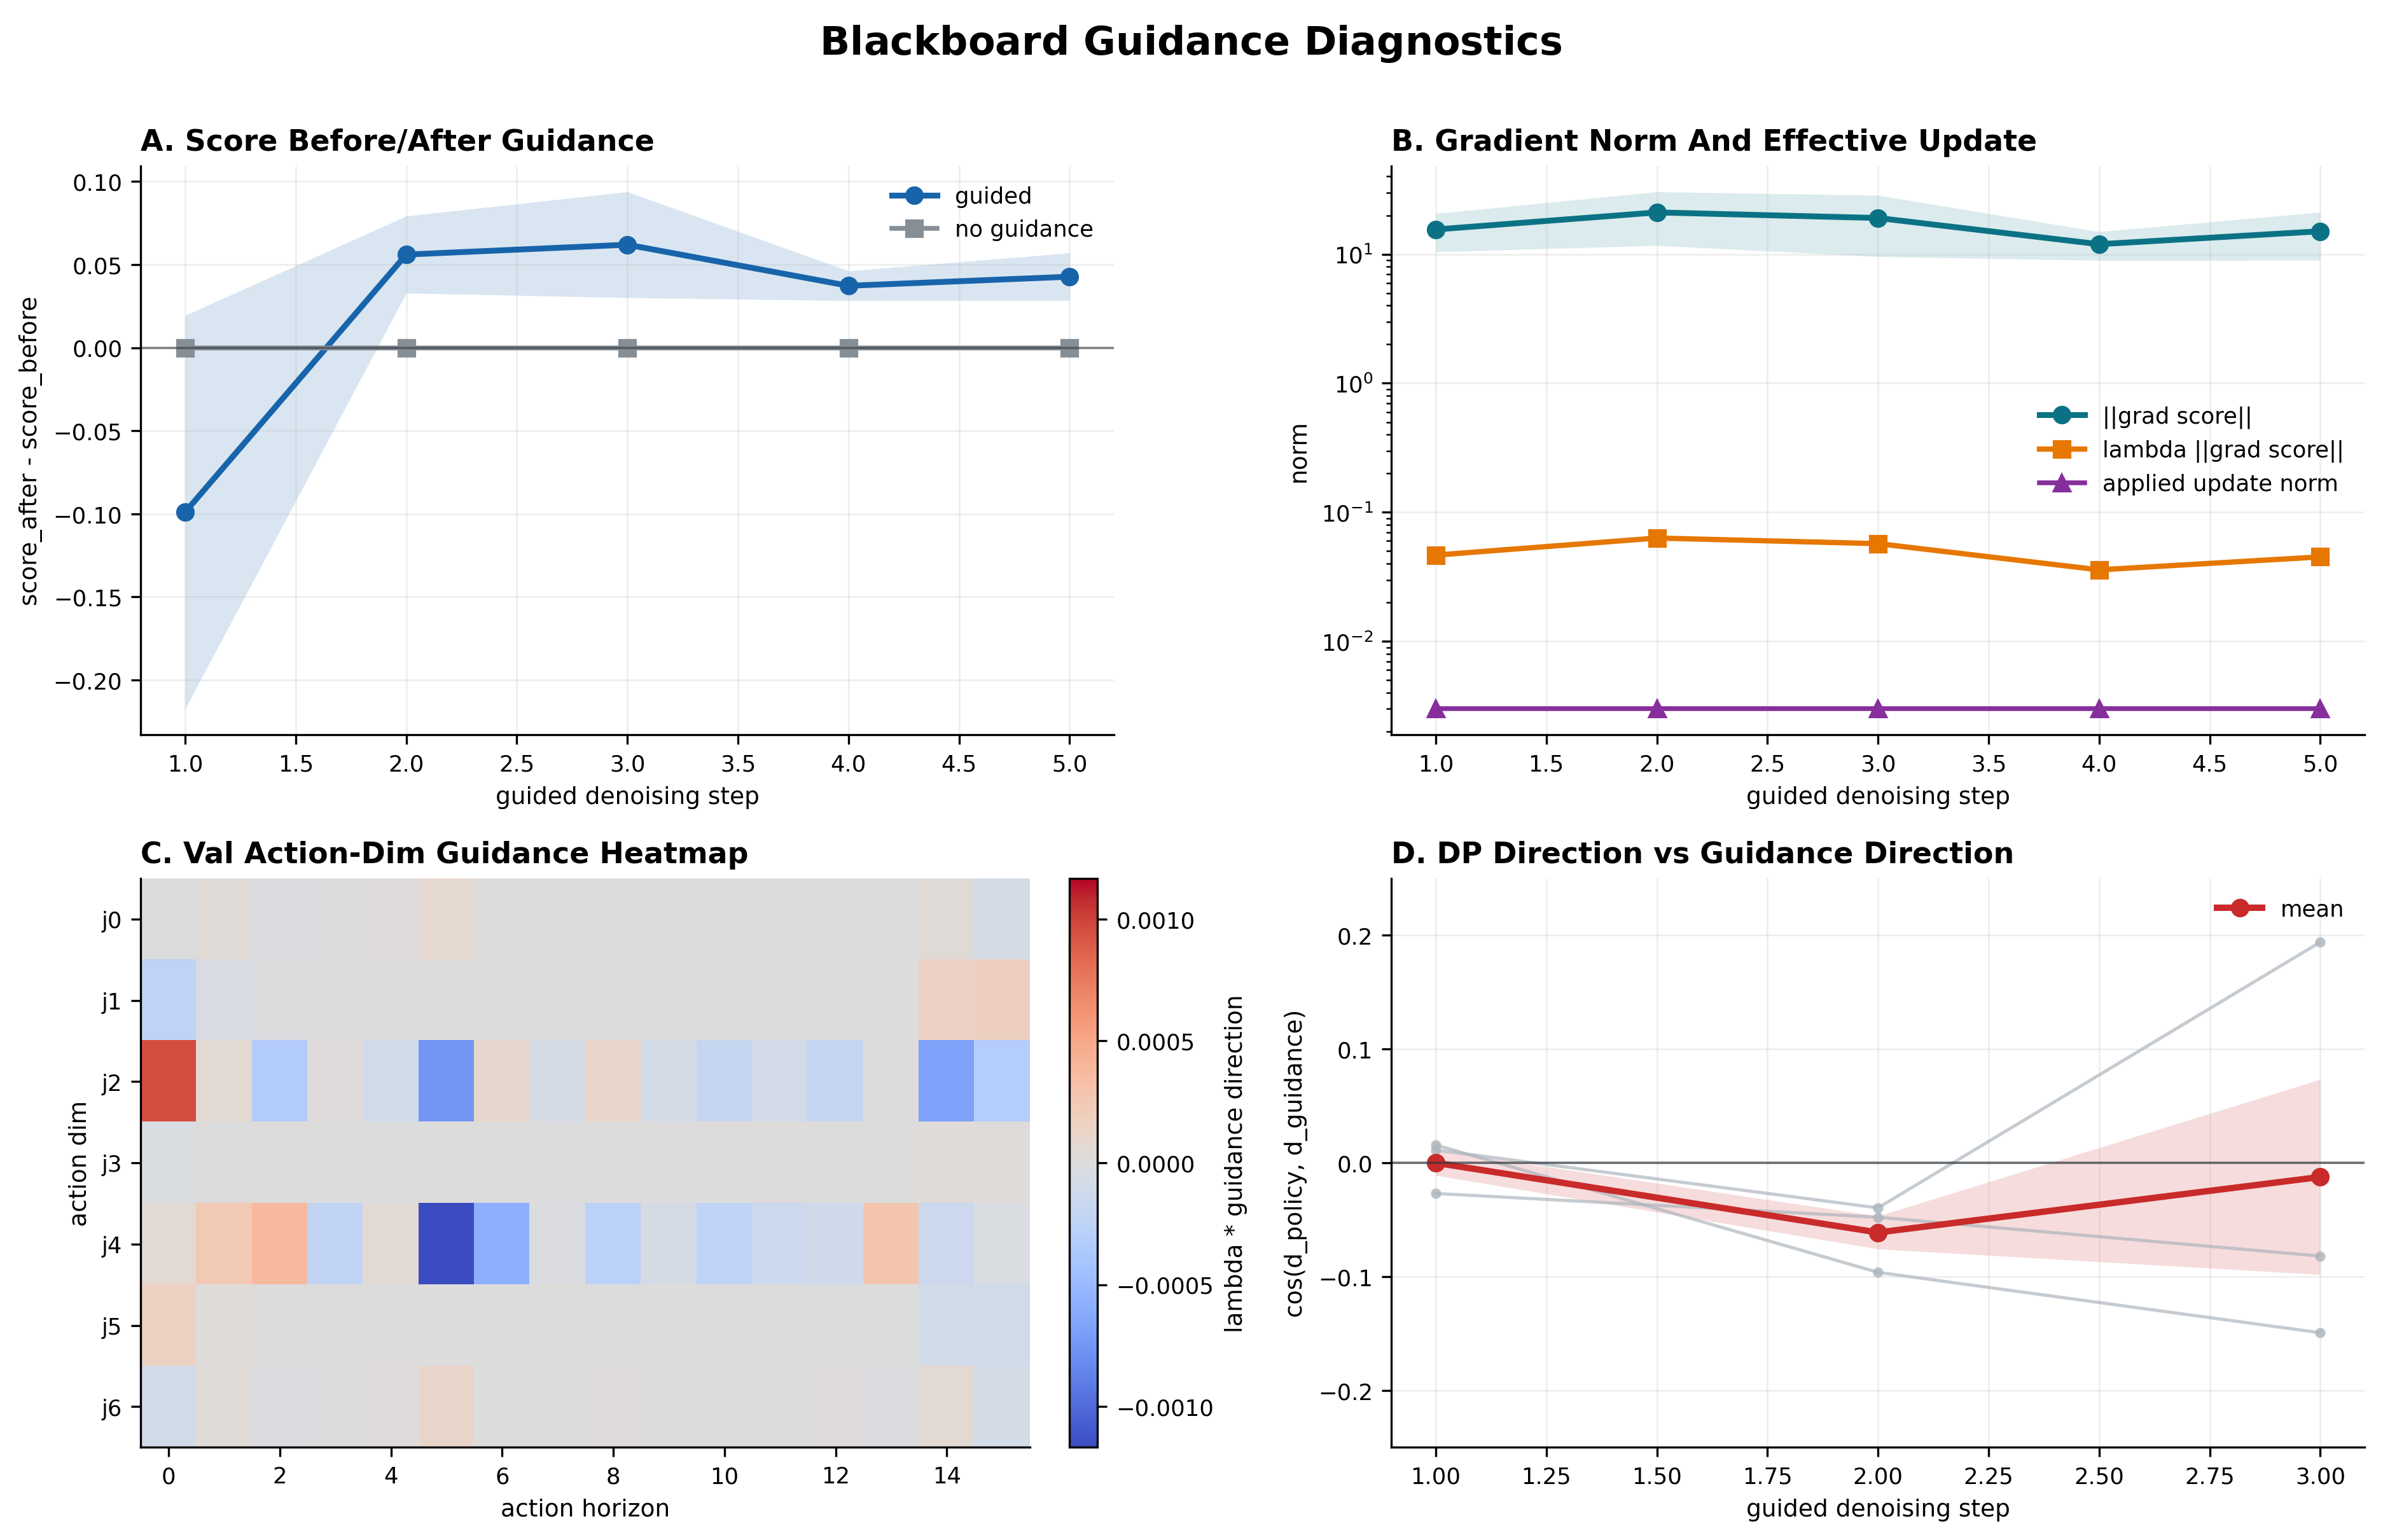
\includegraphics[width=0.92\textwidth]{figures/board_guidance_diagnostics_overview.png}
  \caption{\textbf{Guidance diagnostics for board wiping.} The diagnostic
  analyzes score changes, raw and scaled gradient norms, action-dimension
  localization, and policy-guidance alignment. The evidence supports that
  guidance acts as a small local correction rather than a global trajectory
  rewrite.}
  \label{fig:guidance_diag}
\end{figure*}

\section{ABLATIONS AND FINAL EVALUATION PLAN}

The final submission should include the following ablations.
\textbf{No guidance versus \method{}.} The same DP checkpoint should be run with
guidance disabled and enabled so that the difference isolates inference-time
contact guidance.
\textbf{Reranking versus denoising guidance.} Best-of-$K$ tactile reranking
tests whether the scorer can select better samples; denoising guidance tests
whether the same score can locally improve the current sample.
\textbf{Single-step versus multi-step foresight.} A single endpoint latent tests
whether temporal contact failures can be captured without the full tactile
sequence.
\textbf{Score mode.} The expert margin in (\ref{eq:margin}) should be compared
with raw good-contact probability, clipped energy, and reason-aware energy.
\textbf{Guidance path.} Action-only, tactile-only, and latent-only guidance
separate scorer shortcuts from the intended action-to-foresight-to-score route.

\section{DISCUSSION}

\method{} is motivated by a simple observation: current tactile feedback and
future tactile consequence are different objects. Current tactile feedback is
crucial after contact is observed, but many failures are already implied by the
candidate action before the failure is visible. Predicting future touch creates
a bridge from action choice to contact outcome.

The method also clarifies the role of inference-time optimization. Unbounded
optimization of a learned contact score would be unsafe because the model could
leave the demonstrated action distribution or exploit the scorer. \method{}
therefore uses the base policy as the dominant prior and restricts the contact
score to small late-denoising corrections. The present diagnostics support that
the gradients are finite and localized, but they do not by themselves prove
task improvement. The decisive test remains paired real-robot evaluation using
the same initial conditions and the same base policy weights.

\section{CONCLUSION}

We presented \method{}, a framework for steering robot actions with predicted
contact consequences. The method combines a base diffusion action prior, a
TacVAE tactile latent representation, action-conditioned multi-step tactile
foresight, and a contact-quality energy model whose gradient is applied through
bounded late-denoising guidance. The paper reframes tactile prediction as an
active action-quality signal: the robot predicts what contact an action will
create and locally corrects the action before execution. Current results
validate the representation, foresight, and guidance pathway on the project
tasks. Completing the paired online success-rate and ablation tables is the
remaining requirement before final submission.

\bibliographystyle{IEEEtran}
\bibliography{IEEEabrv,references}

\end{document}
